\section*{Introduction}

ELORank is a C library providing structures and functions implementing the ELO ranking system in a version supporting several players per run with eventual ties.\\ 

It uses the \begin{ttfamily}PBErr\end{ttfamily}, \begin{ttfamily}PBMath\end{ttfamily} and \begin{ttfamily}GSet\end{ttfamily} library.\\

\section{Definitions}

\subsection{ELO rank}

The ELO rank is calculated incrementally by updating the current ELO rank of each entity according to their result in an evaluation process independant from the ELO ranking system. Given a result of this evaluation process, each pair of winner/looser in this result is updated as follow:\\

\begin{equation}
\left\lbrace
\begin{array}{l}
E'_w=E_w+K*\left(1.0-\frac{1.0}{1.0+10.0^{\frac{E_l-E_w}{400.0}}}\right)\\
E'_l=E_l-K*\left(\frac{1.0}{1.0+10.0^{\frac{E_w-E_l}{400.0}}}\right)\\
\end{array}
\right.
\end{equation}

where $K=8.0$ and, $E_w$ and $E_l$ are respectively the current ELO of the winner and the current ELO of the looser and, $E'_w$ and $E'_l$ are respectively the new ELO of the winner and the new ELO of the looser.\\

Tie between two entities results in no changes in their respective ELO rank.

\subsection{Soft ELO rank}

The soft ELO rank is the sliding average of the ELO rank over 100 evaluations:\\
\begin{equation}
softELO(N)=\left\lbrace
\begin{array}{l}
ELO(0)|_{N=0}\\
((N-1)softELO(N-1)+ELO(N))/N|_{N<100}\\
(0.99*(N-1)softELO(N-1)+ELO(N))/100|_{N\geq100}\\
\end{array}
\right.
\end{equation}

where $N\geq0$ is the number of evaluation.

\subsection{Milestone}

A milestone is an entity whose ELO rank is kept unchanged. Any other calculation is performed as usual, but the value of the ELO of this entity isn't updated. A milestone is useful when evaluating a pool of variable entities, for example during the training of a genetic algorithm where the non-elite entities are replaced at each step of the genetic algorithm. By setting the milestone to some cleverly selected entities, one can avoid the "relative" effect of the ELO algorithm and keep a ranking consistent even with respect of entities removed from the ranking. Refer to the Oware example in the MiniFrame repository for an illustration of the use of the milestone property. 

\section{Interface}

\begin{scriptsize}
\begin{ttfamily}
\verbatiminput{/home/bayashi/GitHub/ELORank/elorank.h}
\end{ttfamily}
\end{scriptsize}

\section{Code}

\subsection{elorank.c}

\begin{scriptsize}
\begin{ttfamily}
\verbatiminput{/home/bayashi/GitHub/ELORank/elorank.c}
\end{ttfamily}
\end{scriptsize}

\subsection{elorank-inline.c}

\begin{scriptsize}
\begin{ttfamily}
\verbatiminput{/home/bayashi/GitHub/ELORank/elorank-inline.c}
\end{ttfamily}
\end{scriptsize}

\section{Makefile}

\begin{scriptsize}
\begin{ttfamily}
\verbatiminput{/home/bayashi/GitHub/ELORank/Makefile}
\end{ttfamily}
\end{scriptsize}

\section{Unit tests}

\begin{scriptsize}
\begin{ttfamily}
\verbatiminput{/home/bayashi/GitHub/ELORank/main.c}
\end{ttfamily}
\end{scriptsize}

\section{Unit tests output}

\begin{scriptsize}
\begin{ttfamily}
\verbatiminput{/home/bayashi/GitHub/ELORank/unitTestRef.txt}
\end{ttfamily}
\end{scriptsize}

\section{ELORank.txt}

\begin{scriptsize}
\begin{ttfamily}
\verbatiminput{/home/bayashi/GitHub/ELORank/elorank.txt}
\end{ttfamily}
\end{scriptsize}

\begin{center}
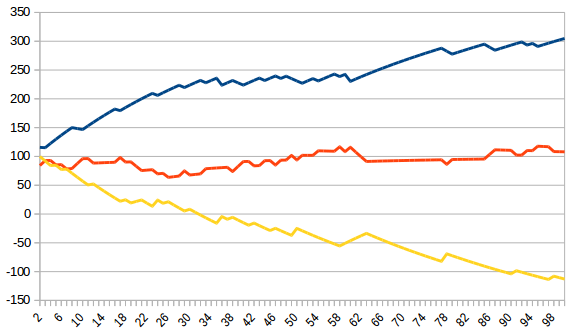
\includegraphics[width=10cm]{elorank.png}
\end{center} 
